\documentclass[svgnames,11pt]{beamer}
\input{/home/tof/Documents/Cozy/latex-include/preambule_commun.tex}
\input{/home/tof/Documents/Cozy/latex-include/preambule_beamer.tex}
\usepackage{pgfpages} \setbeameroption{show notes on second screen=left}
\author[]{Christophe Viroulaud}
\title{Parcours en profondeur\\dans un graphe orienté}
\date{\framebox{\textbf{Algo 18}}}
%\logo{}
\institute{Terminale - NSI}

\begin{document}
\begin{frame}
        \note{\fcolorbox{black}{red}{{\LARGE dfs-annexe.zip}}}
\titlepage
\end{frame}
\begin{frame}
    \frametitle{}

    Dans un graphe non orienté et connexe, tous les sommets sont atteignables depuis n'importe quel sommet de départ.
    \begin{center}
        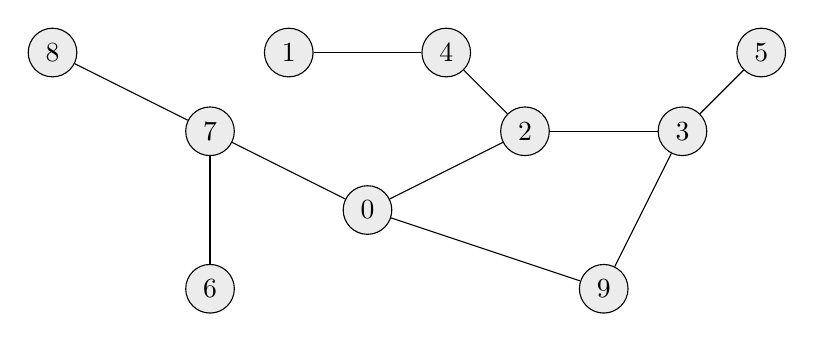
\begin{tikzpicture}
            \node[draw,circle,fill=gray!15] (A)at(0,0) {0};
            \node[draw,circle,fill=gray!15] (B)at(-1,2) {1};
            \node[draw,circle,fill=gray!15] (C)at(2,1) {2};
            \node[draw,circle,fill=gray!15] (D)at(4,1) {3};
            \node[draw,circle,fill=gray!15] (E)at(1,2) {4};
            \node[draw,circle,fill=gray!15] (F)at(5,2) {5};
            \node[draw,circle,fill=gray!15] (G)at(-2,-1) {6};
            \node[draw,circle,fill=gray!15] (H)at(-2,1) {7};
            \node[draw,circle,fill=gray!15] (I)at(-4,2) {8};
            \node[draw,circle,fill=gray!15] (J)at(3,-1) {9};
            \draw[-,>=latex] (E) -- (B);
            \draw[-,>=latex] (A) -- (C);
            \draw[-,>=latex] (A) -- (H);
            \draw[-,>=latex] (A) -- (J);
            \draw[-,>=latex] (H) -- (I);
            \draw[-,>=latex] (H) -- (G);
            \draw[-,>=latex] (C) -- (E);
            \draw[-,>=latex] (C) -- (D);
            %\draw[-,>=latex] (C) -- (J);
            \draw[-,>=latex] (D) -- (J);
            \draw[-,>=latex] (D) -- (F);
        \end{tikzpicture}
    \end{center}

\end{frame}
\begin{frame}
    \frametitle{}

    Dans un graphe orienté, ce n'est pas nécessairement le cas.
    \begin{center}
        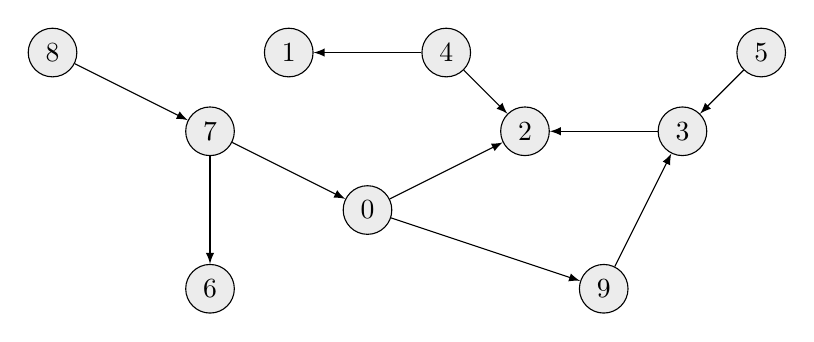
\begin{tikzpicture}
            \node[draw,circle,fill=gray!15] (A)at(0,0) {0};
            \node[draw,circle,fill=gray!15] (B)at(-1,2) {1};
            \node[draw,circle,fill=gray!15] (C)at(2,1) {2};
            \node[draw,circle,fill=gray!15] (D)at(4,1) {3};
            \node[draw,circle,fill=gray!15] (E)at(1,2) {4};
            \node[draw,circle,fill=gray!15] (F)at(5,2) {5};
            \node[draw,circle,fill=gray!15] (G)at(-2,-1) {6};
            \node[draw,circle,fill=gray!15] (H)at(-2,1) {7};
            \node[draw,circle,fill=gray!15] (I)at(-4,2) {8};
            \node[draw,circle,fill=gray!15] (J)at(3,-1) {9};
            \draw[->,>=latex] (E) -- (B);
            \draw[->,>=latex] (A) -- (C);
            \draw[<-,>=latex] (A) -- (H);
            \draw[->,>=latex] (A) -- (J);
            \draw[<-,>=latex] (H) -- (I);
            \draw[->,>=latex] (H) -- (G);
            \draw[<-,>=latex] (C) -- (E);
            \draw[<-,>=latex] (C) -- (D);
            %\draw[-,>=latex] (C) -- (J);
            \draw[<-,>=latex] (D) -- (J);
            \draw[<-,>=latex] (D) -- (F);
        \end{tikzpicture}
        \captionof{figure}{\centering Tous les sommets ne sont pas atteignables depuis \textbf{\texttt{8}}.}
    \end{center}

\end{frame}
\begin{frame}
    \frametitle{}

    \begin{framed}
        \centering Comment réaliser un parcours en profondeur dans un graphe orienté?
    \end{framed}

\end{frame}
\section{Représentation en mémoire}
\begin{frame}
    \frametitle{Représentation en mémoire}

    \begin{center}
        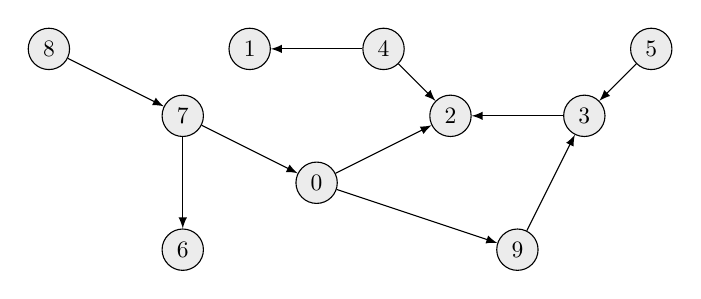
\begin{tikzpicture}[scale=0.85, transform shape]
            \node[draw,circle,fill=gray!15] (A)at(0,0) {0};
            \node[draw,circle,fill=gray!15] (B)at(-1,2) {1};
            \node[draw,circle,fill=gray!15] (C)at(2,1) {2};
            \node[draw,circle,fill=gray!15] (D)at(4,1) {3};
            \node[draw,circle,fill=gray!15] (E)at(1,2) {4};
            \node[draw,circle,fill=gray!15] (F)at(5,2) {5};
            \node[draw,circle,fill=gray!15] (G)at(-2,-1) {6};
            \node[draw,circle,fill=gray!15] (H)at(-2,1) {7};
            \node[draw,circle,fill=gray!15] (I)at(-4,2) {8};
            \node[draw,circle,fill=gray!15] (J)at(3,-1) {9};
            \draw[->,>=latex] (E) -- (B);
            \draw[->,>=latex] (A) -- (C);
            \draw[<-,>=latex] (A) -- (H);
            \draw[->,>=latex] (A) -- (J);
            \draw[<-,>=latex] (H) -- (I);
            \draw[->,>=latex] (H) -- (G);
            \draw[<-,>=latex] (C) -- (E);
            \draw[<-,>=latex] (C) -- (D);
            %\draw[-,>=latex] (C) -- (J);
            \draw[<-,>=latex] (D) -- (J);
            \draw[<-,>=latex] (D) -- (F);
        \end{tikzpicture}
    \end{center}
\begin{activite}
    \begin{enumerate}
        \item Télécharger et extraire le dossier compressé \textbf{\texttt{dfs-annexe.zip}} sur le site \url{https://cviroulaud.github.io}
        \item Créer le fichier \textbf{\texttt{dfs.py}} dans le même dossier que \textbf{\texttt{test.py}}
        \item Construire la matrice \textbf{\texttt{graphe}} des successeurs.
        \item Exécuter le fichier de test pour vérifier la matrice.
    \end{enumerate}
\end{activite}
\end{frame}
\begin{frame}
    \frametitle{Avant de regarder la correction}
\begin{center}
    \centering
    \includegraphics[width=3cm]{/home/tof/Documents/Cozy/latex-include/stop.png}
    \end{center}
{\Large
    \begin{itemize}
        \item Prendre le temps de réfléchir,
        \item Analyser les messages d'erreur,
        \item Demander au professeur.
    \end{itemize}
}
\end{frame}
\begin{frame}[fragile]
    \frametitle{Correction}

\begin{center}
\begin{lstlisting}[language=Python 
     , xleftmargin=2em, xrightmargin=2em]
graphe = [
    [0, 0, 1, 0, 0, 0, 0, 0, 0, 1],
    [0, 0, 0, 0, 0, 0, 0, 0, 0, 0],
    [0, 0, 0, 0, 0, 0, 0, 0, 0, 0],
    [0, 0, 1, 0, 0, 0, 0, 0, 0, 0],
    [0, 1, 1, 0, 0, 0, 0, 0, 0, 0],
    [0, 0, 0, 1, 0, 0, 0, 0, 0, 0],
    [0, 0, 0, 0, 0, 0, 0, 0, 0, 0],
    [1, 0, 0, 0, 0, 0, 1, 0, 0, 0],
    [0, 0, 0, 0, 0, 0, 0, 1, 0, 0],
    [0, 0, 0, 1, 0, 0, 0, 0, 0, 0]]
\end{lstlisting}
\end{center} 

\end{frame}
\section{Parcours en profondeur}
\begin{frame}
    \frametitle{Parcours en profondeur}

    La fonction de parcours en profondeur vue en classe masque un coût: il faut parcourir le tableau \textbf{\texttt{visites}} pour vérifier que le sommet n'a pas déjà été traversé.
    \begin{aretenir}[]
    Une solution classique consiste à créer un tableau \textbf{\texttt{visites}} de booléens. La valeur \textbf{\texttt{False}} à l'indice \textbf{\texttt{i}} indique que le sommet \textbf{\texttt{i}} n'a pas encore été visité.
    
    \end{aretenir}

\end{frame}
\begin{frame}

\begin{activite}
\begin{enumerate}
    \item Construire par compréhension un tableau \textbf{\texttt{visites}}, de la taille  de l'ordre du graphe et rempli de \textbf{\texttt{False}}.
    \item Écrire la fonction \textbf{\texttt{dfs(mat: list, dep: int, vis: list) $\rightarrow$ None}} qui effectue un parcours en profondeur depuis le sommet \textbf{\texttt{dep}}. La fonction affichera, dans la console, les sommets traversés au fur et à mesure du parcours.
    \item Effectuer un parcours en profondeur depuis le sommet \textbf{\texttt{0}}.
\end{enumerate}
\end{activite}

\end{frame}
\begin{frame}
    \frametitle{Avant de regarder la correction}
\begin{center}
    \centering
    \includegraphics[width=3cm]{/home/tof/Documents/Cozy/latex-include/stop.png}
    \end{center}
{\Large
    \begin{itemize}
        \item Prendre le temps de réfléchir,
        \item Analyser les messages d'erreur,
        \item Demander au professeur.
    \end{itemize}
}
\end{frame}
\begin{frame}[fragile]
    \frametitle{Correction}

\begin{center}
\begin{lstlisting}[language=Python , basicstyle=\ttfamily\small, xleftmargin=2em, xrightmargin=2em]
visites = [False for _ in range(len(graphe))]
\end{lstlisting}
\end{center}

\end{frame}
\begin{frame}[fragile]
    \frametitle{Correction}

\begin{center}
\begin{lstlisting}[language=Python , basicstyle=\ttfamily\small, xleftmargin=0.2em, xrightmargin=0em]
def dfs(mat: list, dep: int, vis: list) -> None:
    if not vis[dep]:
        # marque le sommet visités
        vis[dep] = True
        print(dep)
        for i in range(len(mat[dep])):
            # c'est un successeur
            if mat[dep][i] == 1:
                dfs(mat, i, vis)
\end{lstlisting}

\end{center}
\begin{center}
\begin{lstlisting}[language=Python , basicstyle=\ttfamily\small, xleftmargin=0.2em, xrightmargin=0em]
visites = [False for _ in range(len(graphe))]
dfs(graphe, 0, visites)
\end{lstlisting}
\captionof{code}{Appel de la fonction}
\label{CODE}
\end{center}
\end{frame}
\section{Parcours en profondeur de tout le graphe}
\begin{frame}
    \frametitle{Parcours en profondeur de tout le graphe}

    Dans un graphe connexe orienté, tous les sommets ne sont pas forcément atteignables depuis n'importe quel départ. Il faut donc effectuer un parcours depuis chaque sommet.

\end{frame}
\begin{frame}
    \frametitle{}
\begin{activite}
    Écrire la fonction \textbf{\texttt{parcours(mat: list) $\rightarrow$ None}} qui lance un parcours en profondeur depuis chaque sommet. La fonction construira le tableau \textbf{\texttt{visites}} présenté précédemment.
\end{activite}
    

\end{frame}
\begin{frame}
    \frametitle{Avant de regarder la correction}
\begin{center}
    \centering
    \includegraphics[width=3cm]{/home/tof/Documents/Cozy/latex-include/stop.png}
    \end{center}
{\Large
    \begin{itemize}
        \item Prendre le temps de réfléchir,
        \item Analyser les messages d'erreur,
        \item Demander au professeur.
    \end{itemize}
}
\end{frame}
\begin{frame}[fragile]
    \frametitle{Correction}

\begin{center}
\begin{lstlisting}[language=Python , basicstyle=\ttfamily\small, xleftmargin=0.2em, xrightmargin=0em]
def parcours(mat: list) -> None:
    visites = [False for _ in range(len(mat))]
    for i in range(len(mat)):
        # lance un parcours depuis chaque sommet
        dfs(mat, i, visites)
\end{lstlisting}
\end{center}
\begin{center}
\begin{lstlisting}[language=Python , basicstyle=\ttfamily\small, xleftmargin=0.2em, xrightmargin=0em]
parcours(graphe)
\end{lstlisting}
\captionof{code}{Appel de la fonction}
\label{CODE}
\end{center}
\end{frame}
\end{document}